
\pagelayout{wide} % No margins
\addpart{Background}
\labpart{background}
\pagelayout{margin} % Restore margins


\setchapterpreamble[u]{\margintoc}


\chapter{Abstract Interpretation}
\labch{abstract-interpretation}


\marginemptybox{16cm}

In this chapter, we introduce the concepts that are the foundation of this work.
We assume basic knowledge of mathematics, we summarize the necessary background in set theory and logic.
We present an overview of Abstract Interpretation and define the notations and concepts that will be used in the rest of the thesis.

\section{Set Theory}

Here, we briefly revisit well-known concepts to establish the logical and mathematical notation.

\subsection{Logic Notation}

We write $p \defeq P$ to define the mathematical object $p$ to be equal to the object $P$.
Let $\B \defeq \{\true, \false\}$ be the set of Boolean values, where $\true$ represents true and $\false$ represents false.
We can state properties by logical predicates\sidenote{For instance, $x \le x + 1$ is a basic logical predicate}.
We combine predicates using logical connectives: $\land$ for conjunction, $\lor$ for disjunction, $\neg$ for negation, $\implies$ for implication (respectively, $\Leftarrow$ for reverse implication), and $\iff$ for if and only if, as well as $\forall$ for universal and $\exists$ for existential quantification.
In the logical predicate $P \implies Q$, $P$ is called the premise and $Q$ the conclusion.
We call $P$ the \emph{sufficient} condition for $Q$ to hold and, conversely, $Q$ the \emph{necessary} condition for $P$ to hold.
In $P \iff Q$, $P$ is a necessary and sufficient condition for $Q$ to hold, and vice versa.
$P \implies Q$ holds \emph{vacuously} when $P$ is false or when $Q$ is true.
We write $P \defiff Q$ to denote that $P$ is defined to hold whenever $Q$ holds.

\subsection{Sets}


A set $X$ is an unordered collection of distinct elements. We use $x \in X$ (respectively, $x \notin X$) to indicate that $x$ is (respectively, is not) an element of the set $X$. A set is expressed in extension when it is uniquely determined by its elements: \eg, $\{x, y\}$ represents the set containing elements $x$ and $y$. The empty set is denoted by $\emptyset$ and no element belong to it, \ie, $\foralldef{x}{x \notin \emptyset}$.
A singleton $\{x\}$ is a set containing only one element $x$.
A set is defined in comprehension\sidenote{Set comprehension notation will be, in particular, pervasively used in the rest of this thesis.} when its elements are characterized by a common property: $\setdef{x \in X}{P(x)}$ denotes the set of elements $x\in X$ for which $P(x)$ holds.
% In particular, $P$ is a logical predicate that either holds or does not.
% Let $\B \defeq \{\true, \false\}$ be the set of Boolean values, where $\true$ represents true ($P = \true$ means that $P$ holds) and $\false$ represents false ($P = \false$ means that $P$ does not hold).
% We combine predicates using logical connectives: $\land$ for conjunction, $\lor$ for disjunction, $\neg$ for negation, $\implies$ for implication (respectively, $\Leftarrow$ for reverse implication), and $\iff$ for if and only if, as well as $\forall$ for universal and $\exists$ for existential quantification.
% In the logical predicate $P \implies Q$, $P$ is called the premise and $Q$ the conclusion.
% We call $P$ the \emph{sufficient} condition for $Q$ to hold and, conversely, $Q$ the \emph{necessary} condition for $P$ to hold.
% In $P \iff Q$, $P$ is a necessary and sufficient condition for $Q$ to hold, and vice versa.
% $P \implies Q$ holds \emph{vacuously} when $P$ is false or when $Q$ is true.
Contradictions such as circular definitions, \eg, $X \defeq \setdef{x}{x \notin X}$, are avoided in this thesis.
The cardinality of a set $X$ is represented by $\cardinalitynospaces{X}$, \eg, $\cardinalitynospaces{\emptyset} = 0$ and $\cardinalitynospaces{\{x, y\}} = 2$.

A set $X$ is a subset of another set $X'$, denoted $X \subseteq X'$, if every element of $X$ is also an element of $X'$. The empty set $\emptyset$ is subset of any set. The power set $\setof{X}$ of a set $X$ is defined as the set of all the subsets of $X$, \ie, $\setof{X} \defeq \setdef{X'}{X' \subseteq X}$. The union of two sets $X$ and $Y$, denoted $X \setjoin Y$, is the set containing all elements of $X$ and all elements of $Y$, \ie, $X \setjoin Y \defeq \setdef{x}{x \in X \lor x \in Y}$. More generally, the union of a set of sets $X$ is denoted by $\bigsetjoin X$, \ie, $\bigsetjoin X \defeq \bigsetjoin_{X' \in X} X' = \setdef{x}{\existsdef{X' \in X}{x \in X'}}$. The intersection $X \setmeet Y$ of two sets $X$ and $Y$ is the set of all elements that are common to both $X$ and $Y$, \ie, $X \setmeet Y \defeq \setdef{x}{x \in X \land x \in Y}$.
Similarly to the set union, we generalize the intersection to a set of sets $X$ by defining $\bigsetmeet X$ as $\bigsetmeet X \defeq \bigsetmeet_{X' \in X} X' = \setdef{x}{\foralldef{X' \in X}{x \in X'}}$. The relative complement of a set $Y$ in a set $X$, denoted $X \setminus Y$, is the set of all elements of $X$ that are not elements of $Y$, \ie, $X \setminus Y \defeq \setdef{x}{x \in X \land x \notin Y}$. When $Y \subseteq X$ and the set $X$ is clear from the context, we simply write $\neg Y$ for $X \setminus Y$ and we call it the complement of $Y$.
A tuple is an ordered list of elements, \eg, $\langle x_1, \dots, x_n \rangle$ is a tuple of $n$ elements, also called $n$-tuple. Differently from sets, the order of elements in a tuple is significant, \eg, $\langle x, y \rangle \neq \langle y, x \rangle$.
A pair\sidenote{
  Formally, a pair $\tuple{x}{y}$ can be defined as the set $\{\{x\}, \{x, y\}\}$ \cite{Kuratowski1921}.
  Thus, the first coordinate $\tuple{x}{y}_1$ is $z$ such that $\forall X \in \tuple{x}{y}$ it holds that $z \in X$.
  The second coordinate $\tuple{x}{y}_2$ is $z$ such that $\exists X \in \tuple{x}{y}$ such that $z \in X$ and that $\forall X, X' \in \tuple{x}{y}$ it holds that if $X \neq X'$ then $z \notin X$ or $z \notin X'$.
  We have that, $\tuple{x}{y}_1 = x$ and $\tuple{x}{y}_2 = y$.
}\phantomcite{Kuratowski1921} is a tuple of two elements, \eg, $\langle x, y \rangle$ is a pair where the first element is $x$ and the second $y$.
The Cartesian product of two sets $X$ and $Y$, denoted $X \times Y$, is the set of all pairs where the first component is an element of $X$ and the second component is an element of $Y$, \ie, $X \times Y \defeq \setdef{(x, y)}{x \in X \land y \in Y}$.
More generally, $X_1 \times \cdots \times X_n \defeq \setdef{(x_1, \ldots, x_n)}{x_1 \in X_1 \land \cdots \land x_n \in X_n}$ denotes the set of all $n$-tuples from elements of $X_1, \dots, X_n$, and $X^n$ when $X_1 = \cdots = X_n = X$.
The selection of the
$i$-th element of a tuple
$\langle{x_1, \dots, x_n}\rangle$ is denoted by the subscript notation, \ie,
${\langle{x_1, \dots, x_n}\rangle}_i = x_i$ for
$1 \le i \le n$.

A covering of a set $X$ is a set $Z$ of non-empty subsets of $X$ such that every element $x \in X$ belongs to a set in $Z$, \ie, $X = \bigsetjoin Z$. A partition of a set $X$ is a covering $Z$ such that any two sets in $Z$ are disjoint, \ie, every element $x \in X$ belongs to a unique set in $Z$, \ie, $\forall X, Y \in Z : X \neq Y \implies X \setmeet Y = \emptyset$.


\subsection{Numbers}

Let $\N$, $\Z$, and $\R$ be the set of all naturals, integers, and reals, respectively.
In general, whenever the precise numerical type is not known or required, we write $\values\in\{\N, \Z, \R\}$ denoting any possible set of numbers.
We write $\valuesinf$ to denote $\values$ extended with the symbols $-\infty$ and $+\infty$.
The set $\values_{\ge 0}$ denotes the set of non-negative numbers, \ie, $\values_{\ge 0} \defeq \setdef{n \in \values}{n \geq 0}$.
Similarly, we can use this notation with other predicates, for instance, $\values_{\le m} \defeq \setdef{n \in \values}{n \leq m}$ denotes the set of numbers less than or equal to $m$.
As we did not specify whether natural numbers include zero, this notation comes in handy as it permits us to be explicit about the inclusion of zero.
For example, $\N_{\ge 0}^{+\infty}$ denotes the set of natural numbers including zero and $+\infty$, on the other hand, $\N_{> 0}$ denotes the set of strictly positive natural numbers.

Given two bounds $l, u \in \values$, we define the interval $[l, u]$ as the set of numbers between $l$ and $u$, \ie, $[l, u] \defeq \setdef{n \in \values}{l \le n \le u}$. Hence, $[l, u] = \emptyset$ when $l > u$.


\subsection{Relations}
A binary relation $R$ between two sets $X$ and $Y$ is a subset of the cartesian product $X \times Y$.
The following are some important properties which may hold for a binary relation $R$ over a set $S$:
\begin{description}
    \item[Reflexivity]: $\forall x \in S : \tuple{x}{x} \in R$
    \item[Irreflexivity]: $\forall x \in S : \tuple{x}{x} \notin R$
    \item[Symmetry]: $\forall x, y \in S : \tuple{x}{y} \in R \implies \tuple{x}{y} \in R$
    \item[Antisymmetry]: $\forall x, y \in S : \tuple{x}{y} \in R \wedge \tuple{x}{y} \in R \implies x = y$
    \item[Transitivity]: $\forall x, y, z \in S : \tuple{x}{y} \in R \wedge \tuple{y}{z} \in R \implies \tuple{x}{z} \in R$
    \item[Totality]: $\forall x, y \in S : \tuple{x}{y} \in R \vee \tuple{x}{y} \in R$
\end{description}

An \emph{equivalence} relation is a binary relation which is reflexive, symmetric, and transitive. A binary relation which is reflexive (resp. irreflexive), antisymmetric, and transitive is called a \emph{partial order} (resp. \emph{strict partial order}). A \emph{preorder} is reflexive and transitive, but not necessarily antisymmetric. A \emph{total order} is a (strict) partial order which is total, \ie, any two elements of the given set are comparable (\cf{} totality).




\subsection{Ordered Sets}
\labsec{ordered-sets}

A partially ordered set (poset in short) is defined as sets equipped with a partial order relation.

\begin{definition}[Partially Ordered Set]\labdef{poset}
  A \emph{partially ordered set} (poset) $\langle X, \sqsubseteq \rangle$ is a set $X$ equipped with a partial order relation $\sqsubseteq\in\setof{X\times X}$, that is reflexive ($\forall x \in X.\spacer x \sqsubseteq x$), transitive ($\forall x, y, z \in X.\spacer x \sqsubseteq y \land y \sqsubseteq z \implies x \sqsubseteq z$), and antisymmetric ($\forall x, y \in X.\spacer x \sqsubseteq y \land y \sqsubseteq x \implies x = y$).
\end{definition}

\begin{marginfigure}
  \centering
  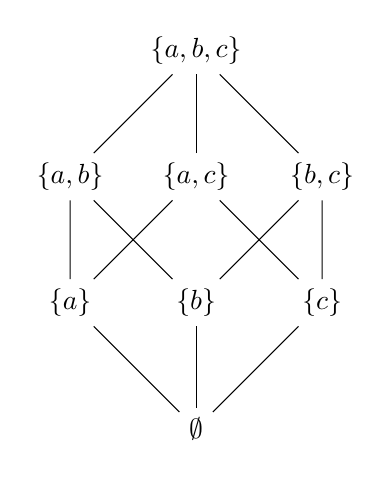
\begin{tikzpicture}[scale=0.8]
    \node (a) at (0,0) {$\emptyset$};
    \node (b) at (-2,2) {$\{a\}$};
    \node (c) at (0,2) {$\{b\}$};
    \node (d) at (2,2) {$\{c\}$};
    \node (e) at (-2,4) {$\{a,b\}$};
    \node (f) at (0,4) {$\{a,c\}$};
    \node (g) at (2,4) {$\{b,c\}$};
    \node (h) at (0,6) {$\{a,b,c\}$};

    \draw (a) -- (b);
    \draw (a) -- (c);
    \draw (a) -- (d);
    \draw (b) -- (e);
    \draw (b) -- (f);
    \draw (c) -- (e);
    \draw (c) -- (g);
    \draw (d) -- (f);
    \draw (d) -- (g);
    \draw (e) -- (h);
    \draw (f) -- (h);
    \draw (g) -- (h);
  \end{tikzpicture}
  \caption{Hasse diagram for the partially ordered set $\langle \setof{\{a, b, c\}}, \subseteq \rangle$.}
  \labfig{hasse_diagram}
  \end{marginfigure}

A finite partially ordered set $\langle D, \sqsubseteq \rangle$ can be represented by a Hasse diagram such as the one in~\reffig{hasse_diagram}: each element $x \in X$ is uniquely represented by a node of the diagram, and there is an edge from a node $x \in X$ to a node $y \in X$ if $y$ covers $x$, that is, $x \sqsubseteq y$ and there exists no $z \in X$ such that $x \sqsubseteq z \sqsubseteq y$. Hasse diagrams are usually drawn placing the elements higher than the elements they cover.

\begin{remark}
  Note that, for \emph{any} set of elements $X$, $\langle X, \subseteq \rangle$ is a poset ordered by set inclusion $\subseteq$.
\end{remark}

\begin{marginfigure}
  \centering
  \begin{tikzpicture}
    \node (a) at (-1,0) {$a$};
    \node (b) at (-2,2) {$b$};
    \node (c) at (0,2) {$c$};

    \draw (a) -- (b);
    \draw (a) -- (c);
  \end{tikzpicture}
  \caption{Hasse diagram for the poset $\langle \setof{a, b, c}, \{(a, b), (a, c)\}\rangle$.}
  \labfig{posetA}
  \end{marginfigure}

\begin{marginfigure}
  \centering
  \begin{tikzpicture}
    \node (a) at (0,0) {$a$};
    \node (b) at (0,2) {$b$};
    \node (c) at (2,0) {$c$};
    \node (d) at (2,2) {$d$};

    \draw (a) -- (b);
    \draw (c) -- (d);
  \end{tikzpicture}
  \caption{Hasse diagram for the poset $\langle \setof{a, b, c, d}, \{(a, b), (c, d)\}\rangle$.}
  \labfig{posetB}
  \end{marginfigure}

\begin{example}
  To draw a few examples: \reffig{posetA} represents the poset $\langle \setof{a, b, c}, \{(a, b), (a, c)\}\rangle$; and \reffig{posetB} represents the poset $\langle \setof{a, b, c, d}, \{(a, b), (c, d)\}\rangle$.
\end{example}

Next we introduce some important concepts related to partially ordered sets.
Let $\langle X, \sqsubseteq \rangle$ be a partially ordered set and $X'$ be a subset of $X$.
\begin{description}
  \item[Greatest Element] When it exists, the greatest element of $X$ (or top) is denoted by $\top$: $\forall x \in X.\spacer x \sqsubseteq \top$.
  \marginnote{Note that, any partially ordered set can always be equipped with a least (resp. greatest) element by adding a new element that is smaller (resp. greater) than every other element.}
  \item[Least Element] When it exists, the least element of $X$ (or bottom) is denoted by $\bot$: $\forall x \in X.\spacer \bot \sqsubseteq x$.
  \item[Maximal Element] An element $x \in X$ is maximal in $X$ if, $\forall y \in X.\spacer x \sqsubseteq y$ implies $x = y$.
  \item[Maximum] A maximal element $x \in X$ is a maximum of $X$ if it is unique.
  \item[Minimal Element] Dually, an element $x \in X$ is minimal in $X$ if, $\forall y \in X.\spacer y \sqsubseteq x$ implies $x = y$.
  \item[Minimum] A minimal element $x \in X$ is a minimum of $X$ if it is unique.
  \item[Upper Bound] An element $x \in X$ is an upper bound of $X'$ if, $\forall y \in X'.\spacer y \sqsubseteq x$.
  \item[Lower Bound] Dually, an element $x \in X$ is a lower bound of $X'$ if, $\forall y \in X'.\spacer x \sqsubseteq y$.
  \item[Least Upper Bound] When it exists, the least upper bound (lub) of $X'$ is denoted by $\join X'$: it is an upper bound $x \in X$ of $X'$ such that, for every upper bound $x' \in X$ of $X'$, $x \sqsubseteq x'$.
  \item[Greatest Lower Bound] When it exists, the greatest lower bound (glb) of $X'$ is denoted by $\meet X'$: it is a lower bound $x \in X$ of $X'$ such that, for every lower bound $x' \in X$ of $X'$, $x' \sqsubseteq x$.
\end{description}

% Let $\langle D, \leq \rangle$ be a partially ordered set. The least element of the poset, when it exists, is denoted by $\bot$: $\forall d \in D : \bot \leq d$. Similarly, the greatest element of the poset, when it exists, is denoted by $\top$: $\forall d \in D : d \leq \top$. Note that any partially ordered set can always be equipped with a least (resp. greatest) element by adding a new element that is smaller (resp. greater) than every other element. Let $X \subseteq D$. A maximal element of $X$ is an element $d \in X$ such that, for each $x \in X$, $x \leq d$. When $X$ has a unique maximal element, it is called maximum and it is denoted by $\max X$. Dually, a minimal element of $X$ is an element $d \in X$ such that, for each $x \in X$, $d \leq x$. When $X$ has a unique minimal element, it is called minimum and it is denoted by $\min X$. An upper bound of $X$ is an element $d \in D$ (not necessarily belonging to $X$) such that, for each $x \in X$, $x \leq d$. The least upper bound (or lub, or supremum) of $X$ is an upper bound $d \in D$ of $X$ and such that, for every upper bound $d' \in D$ of $X$, $d \leq d'$. When it exists, it is unique and denoted by $\bigvee X$ (or $\sup X$). Dually, a lower bound of $X$ is an element $d \in D$ such that, for each $x \in X$, $d \leq x$. The greatest lower bound (or glb, or infimum) of $X$ is a lower bound $d \in D$ of $X$ such that, for every lower bound $d' \in D$ of $X$, $d' \leq d$. When it exists, it is unique and denoted by $\bigwedge X$ (or $\inf X$). Note that the notion of maximal element, maximum, and least upper bound (resp. minimal element, minimum, and greatest lower bound) are different, as illustrated by the following example.

% \begin{example}
% Let us consider the partially ordered set $\langle \setof(\{a, b, c\}), \subseteq \rangle$ represented in \reffig{hasse_diagram} and the subset $X' \defeq \{\{a\}, \{b\}, \{c\}, \{a, b\}, \{a, c\}, \{b, c\}\}$, . The maximal elements of $X$ are $\{a, b\}$, $\{a, c\}$, and $\{b, c\}$. Thus, the maximum $\max X$ of $X$ does not exist, while its least upper bound is $\sup X = \{a, b, c\}$. Similarly, the minimal elements of $X$ are $\{a\}$, $\{b\}$, and $\{c\}$. Thus, the minimum $\min X$ of $X$ does not exist, while its greatest lower bound is $\inf X = \emptyset$.
% \end{example}


\begin{marginfigure}
  \centering
  \begin{tikzpicture}[scale=0.8]
    \node (a) at (0,0) {$\emptyset$};
    \node (b) at (-2,2) {$\{a\}$};
    \node (c) at (0,2) {$\{b\}$};
    \node (d) at (2,2) {$\{c\}$};
    \node (e) at (-2,4) {$\{a,b\}$};
    \node (f) at (0,4) {$\{a,c\}$};
    \node (g) at (2,4) {$\{b,c\}$};
    \node (h) at (0,6) {$\{a,b,c\}$};

    \draw (a) -- (b);
    \draw (a) -- (c);
    \draw (a) -- (d);
    \draw (b) -- (e);
    \draw (b) -- (f);
    \draw (c) -- (e);
    \draw (c) -- (g);
    \draw (d) -- (f);
    \draw (d) -- (g);
    \draw (e) -- (h);
    \draw (f) -- (h);
    \draw (g) -- (h);

    % subset X'
    \draw[seabornBlue, thick, dashed, rounded corners] (-2.9, .7) rectangle (2.9, 5.3);
    \node[seabornBlue] at (3.3, 4.2) {$X'$};

    % maximals of X'
    \draw[seabornGreen, thick, dashed, rounded corners] (-2.7, 3.5) rectangle (2.7, 4.5);
    \node[seabornGreen, fill=white] at (1.8, 4.9) {Maximals};

    % minimals of X'
    \draw[seabornRed, thick, dashed, rounded corners] (-2.7, 1.5) rectangle (2.7, 2.5);
    \node[seabornRed, fill=white] at (-1.8, 1.1) {Minimals};

    % lub of X'
    \draw[seabornYellow, thick, dashed, rounded corners] (-0.4, -0.5) rectangle (0.4, .5);
    \node[seabornYellow, fill=white] at (1, 0) {Lub};

    % glb of X'
    \draw[seabornOrange, thick, dashed, rounded corners] (-0.9, 5.5) rectangle (0.9, 6.5);
    \node[seabornOrange, fill=white] at (1.4, 6) {Glb};
  \end{tikzpicture}
  \caption{Maximal and minimal elements of the subset $X'$, as well as its least upper and greatest lower bounds.}
  \labfig{elements}
  \end{marginfigure}

\begin{example}
  Let us consider the partially ordered set $\langle \setof{\{a, b, c\}}, \subseteq \rangle$ and the subset $X' \defeq \{\{a\}, \{b\}, \{c\}, \{a, b\}, \{a, c\}, \{b, c\}\}$, represented in blue in \reffig{elements}.
  The maximal elements of $X'$ are $\{a, b\}$, $\{a, c\}$, and $\{b, c\}$, labelled ``Maximals'' in green. As we notice, the maximum of $X'$ does not exist, while its least upper bound is $\join X' = \{a, b, c\}$, labelled ``Lub'' in yellow.
  The minimal elements of $X'$ are $\{a\}$, $\{b\}$, and $\{c\}$, labelled ``Minimals'' in red. As we notice, the minimum of $X'$ does not exist, while its greatest lower bound is $\meet X' = \emptyset$, labelled ``Glb'' in orange.
\end{example}



A set equipped with a total order is a \emph{totally ordered set}. A \emph{chain} is a totally ordered subset $Y$ of a poset $\langle X, \sqsubseteq \rangle$. A chain is \emph{ascending} if the sequence of elements is increasing, \ie, $\forall i \in \{1, \ldots, n-1\}.\spacer y_i \sqsubseteq y_{i+1}$, and \emph{descending} if the sequence of elements is decreasing, \ie, $\forall i \in \{1, \ldots, n-1\}.\spacer y_{i+1} \sqsubseteq y_i$. A partially ordered set $\langle X, \sqsubseteq \rangle$ satisfies the \emph{ascending chain condition} if  and only if any infinite ascending chain $y_1 \sqsubseteq y_2 \sqsubseteq \ldots$ has an upper bound in $X$. Dually, it satisfies the \emph{descending chain condition} if and only if any infinite descending chain $y_1 \sqsupseteq y_2 \sqsupseteq \ldots$ has a lower bound in $X$.
A partially ordered set $\langle X, \sqsubseteq \rangle$ is \emph{well-founded} if and only if there are no infinite descending chains without a lower bound in $X$.

\begin{example}
  Let $x!$ be the factorial of $x$, defined as $x! = x \times (x-1) \times \ldots \times 1$ for $x\in\N$.
  The sequence $(x!)_{x\in\N}$ is an infinite ascending chain in the poset $\langle \N, \le \rangle$:
  \[ 1 \le 2 \le 6 \le 24 \le 120 \le \ldots \]
  Hence, the poset $\langle \N, \le \rangle$ does not satisfy the ascending chain condition.
  On the other hand, any possible decreasing chain in $\langle \N, \le \rangle$ has a lower bound, at least $0$, hence it satisfies the descending chain condition and is well-founded.
\end{example}

\marginnote{Note that, since the empty set is a chain, a complete partial order has a least element, \ie, $\bot = \join \emptyset$.}
\begin{definition}[Complete Partial Order]\labdef{cpo}
  A \emph{complete partial order} (CPO) is a partially ordered set $\langle X, \subseteq \rangle$ such that every chain $Y$ has a least upper bound $\join Y$ in $X$.
\end{definition}

As a consequence, any partial ordered set that satisfies the ascending chain condition and is equipped with a least element is a complete partial order.

\subsection{Lattices}
\labsec{lattices}

Lattices are posets that require every nonempty finite subset to have both a least upper bound and a greatest lower bound.

\marginnote{Any totally ordered set is a lattice.}
\begin{definition}[Lattice]\labdef{lattice}
  A \emph{lattice} $\langle X, \sqsubseteq, \join, meet \rangle$ is a poset where $\forall x, x'\in X$ the least upper bound $\join\{x, x'\}$ and the greatest lower bound $\meet\{x, x'\}$ exist.
\end{definition}

Complete lattices are lattices that additionally require every (possibly infinite) subset to have both a least upper bound and a greatest lower bound.

\begin{definition}[Complete Lattice]\labdef{complete-lattice}
  A \emph{complete lattice} $\langle X, \sqsubseteq, \join, \meet, \bot, \top \rangle$ is a lattice where $\forall X' \subseteq X$ the least upper bound $\join X'$ and the greatest lower bound $\meet X'$ exist.
  Complete lattices have both a least element $\bot \defeq \meet X$ and a greatest element $\top \defeq \join X$.
\end{definition}

\begin{marginfigure}
  \centering
  \begin{tikzpicture}
    \node (0) at (0,0) {$0$};
    \node (1) at (0,1) {$1$};
    \node (2) at (0,2) {$2$};
    \node (rest) at (0,3) {$\vdots$};

    \draw (0) -- (1);
    \draw (1) -- (2);
    \draw (2) -- (rest);
  \end{tikzpicture}
  \caption{Hasse diagram for the lattice $\langle \N, \le, \max, \min \rangle$.}
  \labfig{N}
  \end{marginfigure}

\begin{marginfigure}
  \centering
  \begin{tikzpicture}
    \node (0) at (0,0) {$0$};
    \node (1) at (0,1) {$1$};
    \node (2) at (0,2) {$2$};
    \node (rest) at (0,3) {$\vdots$};
    \node (inf) at (0,4) {$+\infty$};

    \draw (0) -- (1);
    \draw (1) -- (2);
    \draw (2) -- (rest);
    \draw (rest) -- (inf);
  \end{tikzpicture}
  \caption{Hasse diagram for the complete lattice $\langle \Nplus, \le, \max, \min, 0, +\infty \rangle$.}
  \labfig{Nplus}
  \end{marginfigure}


\begin{example}
  The posets of \reffig{posetA} and \reffig{posetB} are not lattices, as they do not have a least upper bound for every pair of elements, \eg, $\join\{a, b\}$ does not exist in \reffig{posetA} and $\join\{a, c\}$ does not exist in \reffig{posetB}.
%
  \reffig{hasse_diagram} represents a complete lattice with a finite number of elements.
  The poset $\langle \N, \le \rangle$ is a lattice, as every pair of natural numbers has a least upper bound and a greatest lower bound, but it is not a complete lattice, as $\join \N$ does not exist.
  Lastly, $\langle \Nplus, \le, \max, \min, 0, +\infty \rangle$ where $+\infty$ is greater than any natural number is indeed a complete lattice.
  \reffig{N} shows the Hasse diagram for $\langle \Nplus, \le \rangle$ and \reffig{Nplus} the one for $\langle \Nplus, \le \rangle$.
\end{example}

\begin{remark}
  Given any set of elements $X$, the power set $\langle \setof{X}, \subseteq, \setjoin, \setmeet, \emptyset, X \rangle$ is a complete lattice.
\end{remark}


\subsection{Functions}
\labsec{functions}

% A partial function $f$ from a set $A$ to a set $B$, written $f : A \rightharpoonup B$, is a binary relation between $A$ and $B$ that pairs each element $x \in A$ with no more than one element $y \in B$. The set of all partial functions from a set $A$ to a set $B$ is denoted by $A \rightharpoonup B$. We write $f(x) = y$ if there exists an element $y$ such that $(x, y) \in f$, and we say that $f(x)$ is defined, otherwise we say that $f(x)$ is undefined. Given a partial function $f : A \rightharpoonup B$, we define its domain as $\text{dom}(f) \triangleq \{x \in A \mid \exists y \in B : f(x) = y\}$. The totally undefined function, denoted by $\emptyset$, has the empty set as domain: $\text{dom}(\emptyset) = \emptyset$. The join of two partial functions $f_1 : A \rightharpoonup B$ and $f_2 : A \rightharpoonup B$ with disjoint domains, denoted by $f_1 \cup f_2 : A \rightharpoonup B$, is defined as follows:
% \[
% (f_1 \cup f_2)(x) \triangleq
% \begin{cases}
% f_1(x) & x \in \text{dom}(f_1) \\
% f_2(x) & x \in \text{dom}(f_2) \\
% \text{undefined} & \text{otherwise}
% \end{cases}
% \]
% where $\text{dom}(f_1) \cap \text{dom}(f_2) = \emptyset$.

% A (total) function $f$ from a set $A$ to a set $B$, written $f : A \to B$, is a partial function that pairs each $x \in A$ with exactly one element $y \in B$. Equivalently, a (total) function $f : A \to B$ is a partial function such that $\text{dom}(f) = A$. The set of all functions from a set $A$ to a set $B$ is denoted by $A \to B$.

% We sometimes denote functions using the lambda notation $\lambda x \in A. f(x)$, or more concisely $\lambda x. f(x)$.

% The composition of two functions $f : A \to B$ and $g : B \to C$ is another function $g \circ f : A \to C$ such that $\forall x \in A : (g \circ f)(x) = g(f(x))$.

% The following properties may hold for a function $f : A \to B$:
% \begin{itemize}
%     \item Injectivity: $\forall x, y \in A : f(x) = f(y) \implies x = y$
%     \item Surjectivity: $\forall y \in B : \exists x \in A : f(x) = y$
% \end{itemize}

% A bijective function, also called isomorphism, is both injective and surjective. Two sets $A$ and $B$ are isomorphic if there exists a bijective function $f : A \to B$. The inverse of a bijective function $f : A \to B$ is the bijective function $f^{-1} : B \to A$ defined as $f^{-1} \triangleq \{(b, a) \mid (a, b) \in f\}$.

% Let $\langle D_1, \leq_1 \rangle$ and $\langle D_2, \leq_2 \rangle$ be partially ordered sets. A function $f : D_1 \to D_2$ is said to be monotonic when, for each $x, y \in D_1, x \leq_1 y \implies f(x) \leq_2 f(y)$. It is continuous (or Scott-continuous) when it preserves existing least upper bounds of chains, that is, for each chain $C \subseteq D_1$, if $\bigvee C$ exists then $f(\bigvee C) = \bigvee \{f(x) \mid x \in C\}$. Dually, it is co-continuous when it preserves existing greatest lower bounds of chains, that is, if $\bigwedge C$ exists then $f(\bigwedge C) = \bigwedge \{f(x) \mid x \in C\}$. A complete $\bigvee$-morphism (resp. complete $\bigwedge$-morphism) preserves existing least upper bounds (resp. greatest lower bounds) of arbitrary non-empty sets.

% Given a complete lattice $\langle D, \leq, \bigvee, \bigwedge, \bot, \top \rangle$ (resp. a lattice, a cpo, a poset) and a set $S$, the set $S \to D$ of all functions from $S$ to $D$ inherits the complete lattice (resp. lattice, cpo, poset) structure of $D$: $\langle S \to D, \leq, \bigvee, \bigwedge, \bot, \top \rangle$ where the dotted operators are defined by pointwise lifting:
% \[
% \begin{aligned}
% f \leq g & \triangleq \forall s \in S : f(s) \leq g(s) \\
% \bigvee X & \triangleq \lambda s. \bigvee \{f(s) \mid f \in X\} \\
% \bigwedge X & \triangleq \lambda s. \bigwedge \{f(s) \mid f \in X\} \\
% \bot & \triangleq \lambda s. \bot \\
% \top & \triangleq \lambda s. \top
% \end{aligned}
% \]

A \emph{function} is a relation $f\in\setof{X \times Y}$ between two sets $X$ and $Y$ such that each element $x \in X$ is in relation with at most one element $y \in Y$, \ie, $\forall x \in X.\spacer \exists! y \in Y.\spacer (x, y) \in f$. We write $f \in X \to Y$ to denote that $f$ is a function from $X$ to $Y$, and $f(x) = y$ if and only if $\langle x, y \rangle \in f$.
We sometimes denote functions using the \emph{lambda notation} $\lambda x \in X.\spacer f(x)$, or more concisely $\lambda x.\spacer f(x)$ when the domain is clear from the context.
The \emph{domain} of a function $f$ is the set of elements $x \in X$ such that $f(x)$ is defined, \ie, $\dom(f) \defeq \setof{x \in X \mid \exists y \in Y.\spacer f(x) = y}$. Dually, the \emph{codomain} of a function $f$ is the set of elements $y \in Y$ such that there exists $x \in X$ such that $f(x) = y$, \ie, $\codom(f) \defeq \setof{y \in Y \mid \exists x \in X.\spacer f(x) = y}$. A function $f$ is \emph{total} when $\dom(f) = X$, otherwise \emph{partial} when $\dom(f) \subseteq X$.
A function $f\in X \to X$ is called an \emph{operator} when the domain and codomain coincide.

The {composition} of two functions $f \in X \to Y$ and $g \in Y \to Z$ is the function $g \circ f \in X \to Z \defeq \lambda x.\spacer g(f(x))$.
The {iterates} of an operator $f \in X \to X$ are defined as $f^0 \defeq \identity$ and $f^{n+1} \defeq f \circ f^n$ for $n \in \N$.
We define the {identity} function $\identity\in X \to X$ as $\identity \defeq \lambda x.\spacer x$.
Let $f \in X \to Y$ be a function, the following properties may hold for $f$:
\begin{description}
  \item[Injectivity] $\forall x, y \in X.\spacer f(x) = f(y) \implies x = y$.
  \item[Surjectivity] $\forall y \in Y.\spacer \exists x \in X.\spacer f(x) = y$.
  \item[Bijectivity] A function that is both injective and surjective is called bijective, or isomorphism.
\end{description}
Two sets $X$ and $Y$ are \emph{isomorphic} if there exists a bijective function $f \in X \to Y$.
%
Next, we introduce some properties of functions that are relevant in the context of partially ordered sets.

\begin{definition}[Monotonicity]\labdef{monotonicity}
  Let $f\in X \to Y$ be a function, $\langle X, \sqsubseteq_X \rangle$ and $\langle Y, \sqsubseteq_Y \rangle$ be two partially ordered sets.
  The function $f$ is \emph{monotonic} whenever, for all $x, x' \in X$, it holds that $x \sqsubseteq_X x' \implies f(x) \sqsubseteq_Y f(x')$.
\end{definition}

Sometimes we refer to a function as \emph{increasing} monotone when it is monotonic and \emph{decreasing} monotone when it is monotonic and the inequality is reversed, \ie, $x \sqsubseteq_X x' \implies f(x') \sqsupseteq_Y f(x)$. Note that, a decreasing monotone function is (increasing) monotone over $\langle X, \sqsubseteq_Y \rangle$ and $\langle Y, \sqsupseteq_Y \rangle$.

\begin{definition}[Continuity]\labdef{continuity}
  Let $f\in X \to Y$ be a function, $\langle X, \sqsubseteq_X, \join_X, \meet_X \rangle$ and $\langle Y, \sqsubseteq_Y, \join_Y, \meet_Y \rangle$ be two partially ordered sets.
  The function $f$ is \emph{continuous} (or \emph{Scot-continuous}) whenever, for all chains $C \subseteq X$, if $\join_X C$ exists then the limit coincide, \ie, $f(\join_X C) = \join_Y \setof{f(x) \mid x \in C}$.
\end{definition}

Dually, a function is \emph{co-continuous} whenever, for all chains $C \subseteq X$, if $\meet_X C$ exists then the limit coincide, \ie, $f(\meet_X C) = \meet_Y \setof{f(x) \mid x \in C}$. A \emph{complete $\join$-morphism} (resp. \emph{complete $\meet$-morphism}) preserves existing least upper bounds (resp. greatest lower bounds) of arbitrary non-empty sets.

% The upper closure of a subset $Y\subseteq X$ in a poset $\langle X, \sqsubseteq\rangle$ is the set of all elements in $X$ that are greater than or equal to some element of $Y$.
% We write $\uparrow Y \defeq \setdef{x \in X}{\exists y \in Y.\spacer y \sqsubseteq x}$ for the upper closure of $Y$. Dually, the lower closure of a subset $Y\subseteq X$ in a poset $\langle X, \sqsubseteq\rangle$ is the set of all elements in $X$ that are smaller than or equal to some element of $Y$, and is denoted by $\downarrow Y \defeq \setdef{x \in X}{\exists y \in Y.\spacer x \sqsubseteq y}$.

An operator is \emph{idempotent} when $f(f(x)) = f(x)$ for all $x \in X$, and \emph{extensive} when $x \sqsubseteq f(x)$ for all $x \in X$.

\begin{definition}[Upper Closure Operator]\labdef{upper-closure-operator}
  An \emph{upper closure operator} on a partially ordered set $\langle X, \subseteq \rangle$ is an operator $\rho\in X \to X$ which is monotone, idempotent, and extensive.
\end{definition}

A \emph{family} $F \in \Delta \to X$ of elements of $X$ indexed by a set $\Delta$ (called the \emph{domain} or \emph{indexed set} of $F$, which may be infinite) is a function from $\Delta$ to $X$. Such family defines a set $\setdef{F(i)}{i \in \Delta}$ (where $F(i)$ is often denoted as $F_i$ with an index $i\in\Delta$) of elements of $X$ indexed by $\Delta$.
It also defines the sequence $(F_i)_{i\in\Delta}$ of elements of $X$ indexed by $\Delta$.

\begin{example}
  Let $\textsc{fib}(n)$ be the $n$-th Fibonacci number, defined as:
  \begin{align*}
    \textsc{fib}(n) \defeq \begin{cases}
      n & \text{if } n \le 1 \\
      \textsc{fib}(n-1) + \textsc{fib}(n-2) & \text{otherwise}
    \end{cases}
  \end{align*}
  The sequence $(\textsc{fib}(n))_{n\in\N}$ is a family of elements of $\N$ indexed by $\N$:
  \[ 0, 1, 1, 2, 3, 5, 8, 13, 21, 34, \ldots \]
\end{example}

\subsection{Properties}
\labsec{properties}

Properties (\eg, ``to be an even natural number'' or ``to be a number of the sequence of Fibonacci'') by extension are the sets of elements that satisfy the property (\eg, $2\N \defeq \setdef{x \in \N}{\exists k \in \N.\spacer x = 2k}$ or $B \defeq \setdef{\textsc{fib}(n)}{n\in\N}$). Therefore, if $Q$ is a property, then $x \in Q$ means that $x$ satisfies the property $Q$ (\eg, $2 \in 2\N$ or $12 \notin B$).

By considering properties as sets, we have that logical implication is subset inclusion. For instance, the property ``to be an even natural number'' implies ``to be a multiple of $4$'', that is $2\N \subseteq 4\N$, where $4\N \defeq \setdef{x \in \N}{\exists k \in \N.\spacer x = 4k}$.
Whenever $P$ implies $Q$ ($P \subseteq Q$), we say that $P$ is \emph{stronger} than $Q$ and $Q$ is \emph{weaker} than $P$.
Stronger properties are satisfied by less elements, whether weaker properties are satisfied by more.
The strongest property is $\emptyset$ satisfied by no element, and the weakest property is the set containing all elements, \eg, $\N$ is the weakest property of natural numbers.


\subsection{Fixpoints}
\labsec{fixpoints}

Fixpoints are elements of a poset that are invariant under a function.
As of fundamental importance to formally reason about program behaviors, we introduce the concept of fixpoints in partially ordered sets.
In the following, let $\langle X, \subseteq \rangle$ be a partially ordered set and $f : X \to X$ be an operator on $X$.

\begin{description}
  \item[Fixpoint] An element $x \in X$ is a \emph{fixpoint} of $f$ whenever $f(x) = x$.
  \item[Prefixpoint] An element $x \in X$ is a \emph{prefixpoint} of $f$ whenever $x \sqsubseteq f(x)$.
  \item[Postfixpoint] An element $x \in X$ is a \emph{postfixpoint} of $f$ whenever $f(x) \sqsubseteq x$.
  \item[Set of Fixpoints] The set of fixpoints of $f$ is denoted by $\fixpoints(f) \defeq \setdef{x \in X}{f(x) = x}$.
  \item[Least Fixpoint] The \emph{least fixpoint} of $f$ is a fixpoint of $f$ such that, for every fixpoint $x \in X$ of $f$, $\lfp f \sqsubseteq x$. We write $\lfp_{x_0} f$ for the least fixpoint of $f$ which is greater than or equal to $x_0 \in X$.
  \item[Greatest Fixpoint] The \emph{greatest fixpoint} of $f$ is a fixpoint of $f$ such that, for every fixpoint $x \in X$ of $f$, $x \sqsubseteq \gfp f$. We write $\gfp_{x_0} f$ for the greatest fixpoint of $f$ which is smaller than or equal to $x_0 \in X$.
\end{description}

When the order $\sqsubseteq$ is not clear from the context, we explicitly write $\lfp^{\sqsubseteq} f$ and $\gfp^{\sqsubseteq} f$. Note that, in general, a function may have no fixpoint at all or multiple ones.

\begin{marginfigure}
% simple plot x-y axis for the fibonacci function
% grid system showing the fixpoints
\begin{tikzpicture}[scale=0.65]
  \begin{axis}[
    grid=both,
    major grid style = {dashed, lightgray},  % Style for major grid lines
    minor grid style = {dashed, gray!25},    % Style for minor grid lines
    xtick = {0, 1, 2, 3, 4, 5, 6},% x-axis ticks
    ytick = {0, 1, 2, 3, 5, 8},  % y-axis ticks (Fibonacci numbers)
    xmin = 0, xmax = 6.5,
    ymin = 0, ymax = 8.5]
    \addplot[samples at={0,1,...,6},only marks, seabornBlue] {( ((1+sqrt(5))/(2))^\x - cos(deg(\x * pi)) * ((1+sqrt(5))/(2))^(-\x) )/sqrt(5) };
    \addplot[domain=0:6.5, seabornRed, thick] {x};
  \end{axis}

  \draw[seabornYellow, thick, dashed, rounded corners] (-0.4, -0.5) -- (0.2, -0.5) -- (4, 3) -- cycle;
  % \node[seabornYellow, fill=white] at (1, 0) {Lub};
\end{tikzpicture}
\caption{Fixpoints of the fibonacci function.}
\labfig{fixpoints}
\end{marginfigure}

\begin{example}
  Let us consider again the fibonacci function $\textsc{fib} \in \N \to \N$. The fixpoints are shown in \reffig{fixpoints}, the set of fixpoints is $\fixpoints(\textsc{fib}) = \setof{0, 1, 5}$, the elements $2$, $3$, and $4$ are prefixpoints are their values are smaller than the values of their images, and the elements greater than or equal to $6$ are postfixpoints.
  The least fixpoint of $\textsc{fib}$ is $\lfp \textsc{fib} = 0$, as $0$ is the smallest element of $\fixpoints(\textsc{fib})$.
  On the other hand, the greatest fixpoint of $\textsc{fib}$ is $\gfp \textsc{fib} = 5$.

  Instead, if we consider another operator, for example the $\textsc{cons}(x) \defeq x + 1$ operator, then there is no fixpoint, as $\textsc{cons}(x) \neq x$ for all $x \in \N$.
\end{example}

Next, we recall a fundamental theorem of Alfred Tarski \sidecite{Tarsky1955} that characterizes fixpoints of monotonic functions over complete lattices.

\begin{theorem}[Tarski's Fixpoint Theorem]\labthm{tarski}
  Let $\langle X, \sqsubseteq, \join, \meet, \bot, \top \rangle$ be a complete lattice and $f \in X \to X$ be a monotonic function. The set of fixpoints $\fixpoints(f)$ is a non-empty complete lattice.
\end{theorem}
\begin{proof}
  See \textcite{Tarsky1955}.
\end{proof}
\refthm{tarski} guarantees that $f$ has a least fixpoint $\lfp f = \meet \setdef{x \in X}{f(x) \sqsubseteq x}$ and a greatest fixpoint $\gfp f = \join \setdef{x \in X}{x \sqsubseteq f(x)}$ as $fixpoints(f)$ is a non-empty complete lattice.

However, such characterization is not constructive, an alternative that expresses the least fixpoint of a function as the limit of iterates is Kleene's Fixpoint Theorem \sidecite{Kleene1952}.


\marginnote{
  In case of monotonic but not continuous functions, a theorem by Patrick and Radhia Cousot \cite{Cousot1979b} expresses fixpoints as the limit of possibly transfinite iterations.
}\phantomcite{Cousot1979b}
\begin{theorem}[Kleene's Fixpoint Theorem]\labthm{kleene}
  Let $\langle X, \sqsubseteq \rangle$ be a complete partial order and $f \in X \to X$ be a Scott-continuous function. The least fixpoint $\lfp f$ exists and is the least upper bound of the iterates $f^n$ starting from $\bot$:
  \[ \lfp f = \join \setdef{f^n(\bot)}{n \in \N} \]
\end{theorem}

In the following, the partial order between the fixpoint iterates is called the \emph{computational order}, in order to distinguish it from the \emph{approximation order} defined in the next section.

\section{Notations of Abstract Interpretation}
\labsec{notations-of-abstract-interpretation}

\emph{Abstract Interpretation} \sidecite{Cousot1977,Cousot1978} is a general theory for approximating the semantics of programs as a unifying framework for static program analysis, co-invented in the late 1970s by Patrick and Radhia Cousot.
In the following, we introduce the notations, main definitions, and results that will be used throughout the rest of this thesis.

\subsection{Transition System}
\labsec{transition-system}

The \emph{semantics} of a program is a mathematical characterization of its behavior for all possible input data.
In order to be independent of a particular choice of programming language, we consider programs as transition systems, where the behavior of a program is described by a set of states and a set of transitions between states.
In the next section, we instantiate the transition system model for a small imperative language.

\begin{definition}[Transition System]\labdef{transition-system}
  A \emph{transition system} is a pair $\transitionsystem$ where $\state$ is a (potentially infinite) set of states and $\transitionrelation \in \transitionrelationtype$ is the transition relation.
\end{definition}

This model allows expressing programs with (possibly unbounded) non-determinism.
In the following, we write $\defstate \rightarrow \defstate'$ to denote that there is a transition from state $\defstate$ to state $\defstate'$, \ie, $\tuple{\defstate}{\defstate'} \in \transitionrelation$.
The set $\finalstates \defeq \setdef{\defstate \in \state}{\forall \defstate' \in \state.\spacer \tuple{\defstate}{\defstate'} \notin \transitionrelation}$ represents the \emph{final states} (or blocking states) of the transition system.


\subsection{Maximal Trace Semantics}
\labsec{maximal-trace-semantics}

The \emph{semantics} of a program is a mathematical characterization of its behavior for all possible input data. We formally define this notion for a transition system below.

\paragraph{Sequences.}
Given a set of elements $X$, the set of all sequences of exactly $n$ elements of $X$ is denoted by $X^n\defeq\setdef{\defstate_0 \dots \defstate_{n-1}}{\forall i < n.\spacer s_i \in X}$.
The symbol $\emptysequence$ denotes the empty sequence, hence $X^0 = \{\emptysequence\}$.

We define:
\begin{description}
  \item[Finite Sequences $\retrievefiniteoremptytraces{X}$:] The set of all finite sequences of elements of $X$ is defined as $\retrievefiniteoremptytraces{X} \defeq \bigsetjoin_{n \in \N} X^n$.
  \item[Non-Empty Finite Sequences $\retrievefinitetraces{X}$:] The set of all non-empty finite sequences of elements of $X$ is $\retrievefinitetraces{X} \defeq \retrievefiniteoremptytraces{X} \setminus X^0 = \bigsetjoin_{n \in \Nposstrict} X^n$.
  \item[Infinite Sequences $\retrieveinfinitetraces{X}$:] The set of all infinite sequences of elements of $X$ is defined as  $\retrieveinfinitetraces{X} \defeq \setdef{\defstate_0 \dots}{\forall i \in \N.\spacer \defstate_i \in X}$.
  \item[Non-Empty Finite or Infinite Sequences $\retrievefiniteinfinitetraces{X}$:] The set of all non-empty finite or infinite sequences of elements of $X$ is $\retrievefiniteinfinitetraces{X} \defeq \retrievefinitetraces{X} \cup \retrieveinfinitetraces{X}$.
  \item[Finite or Infinite Sequences $\retrievefiniteoremptyinfinitetraces{X}$:] The set of all finite or infinite sequences of elements of $X$ is $\retrievefiniteoremptyinfinitetraces{X} \defeq \retrievefiniteoremptytraces{X} \cup \retrieveinfinitetraces{X}$.
\end{description}

Let $\defstate\in X$ be an element, we often refer to just $\defstate$ as the sequence of length $1$ containing only $\defstate$, \ie, $\{\defstate\} \in X^1$.
To \emph{concatenate} two sequences $\defseq, \defseq' \in \retrievefiniteinfinitetraces{X}$, we write $\concat{\defseq}{\defseq'}$ for the sequence obtained by appending $\defseq'$ to $\defseq$. It holds that $\concat{\defseq}{\emptysequence} = \concat{\emptysequence}{\defseq} = \defseq$ and $\concat{\defseq}{\defseq'} = \defseq$ whenever $\defseq \in \retrieveinfinitetraces{X}$. To \emph{merge} two set of sequences $Y \subseteq \retrievefinitetraces{X}$ and $Y' \subseteq \retrievefiniteinfinitetraces{X}$, we write $\mergesequences{Y}{Y'} \defeq \setdef{\concat{\defseq}{\concat{\defstate}{\defseq'}}}{\defstate \in X \land \concat{\defseq}{\defstate} \in Y \land \concat{\defstate}{\defseq'} \in Y'}$ when a finite sequence in $Y$ ends with the initial state of a sequence in $Y'$.

\paragraph{Traces.}

Given a transition system $\transitionsystem$, a \emph{trace} is a non-empty sequence of program states $\state$ that respects the transition relation $\transitionrelation$. That is, for every pair of consecutive states $\defstate, \defstate' \in \state$, it holds that $\tuple{\defstate}{\defstate'} \in \transitionrelation$.

\paragraph{Maximal Trace Semantics}

The \emph{maximal trace semantics} $\tracesemanticsnoparam\in\tracetype$ of a transition system $\transitionsystem$ is the set of all traces that are terminating in the final states $\finalstates$ (\ie, of finite length) and all non-terminating traces (\ie, of infinite length) generated by $\transitionsystem$.


\begin{definition}[Maximal Trace Semantics]\labdef{maximal-trace-semantics}
  Let $\transitionsystem$ be a transition system. The \emph{maximal trace semantics} $\tracesemanticsnoparam\in\tracetype$ generated by $\transitionsystem$ is defined as:
  \begin{align*}
    \tracesemanticsnoparam \DefeQ &\bigsetjoin_{n\in\Nposstrict} \setdef{s_0\dots s_{n-1}\in\finitetontraces}{\foralldef{i < n-1}{\tuple{s_i}{s_{i+1}}\in\transitionrelation \land s_{n-1}\in \finalstates}} \\
    &\setjoin \setdef{s_0\dots{}\in\infinitesequences}{\foralldef{i\in\N}{\tuple{s_i}{s_{i+1}}\in\transitionrelation}}
  \end{align*}
\end{definition}

\begin{example}
  Let us consider the transition system $\transitionsystem$ with states $\state = \{x, y\}$, transitions $\transitionrelation = \{\tuple{x}{x}, \tuple{x, y}\}$ with final states $\finalstates = \{y\}$. The maximal trace semantics $\tracesemanticsnoparam$ is the set of all traces that are terminating in the final state $y$ and all non-terminating traces from the transition $\tuple{x}{x}$.
  That is, $\tracesemanticsnoparam = \retrieveinfinitetraces{x} \setjoin {\retrievefiniteoremptytraces{x}}{y}$.
  Note that, the maximal trace semantics does not represent partial computations that are not terminating in the final states, such as the trace $\{x\spacer x\spacer x\}$.
\end{example}

\begin{remark}
  Observe that not all program semantics can be generated by a transition system. For instance, in case the program semantics is the set of traces $\retrievefiniteoremptytraces{x}y$ where $y$ is eventually reached, the transition relation $\transitionrelation = \{\tuple{x}{x}, \tuple{x}{y}\}$ generates also infinite sequences of $x$ that are not part of the semantics.
\end{remark}

The following result provides a (least) fixpoint characterization of the maximal trace semantics over the complete lattice $\tracecompletelattice$.
The \emph{computation order} of the maximal trace semantics is defined as $\defsetoftraces \tracesubseteq \defsetoftraces' \defiff \retrievefinitetraces{\defsetoftraces} \subseteq \retrievefinitetraces{\defsetoftraces'} \land \retrieveinfinitetraces{\defsetoftraces} \supseteq \retrieveinfinitetraces{\defsetoftraces'}$.

\begin{theorem}[Maximal Trace Semantics]\labthm{maximal-trace-semantics}
  The \emph{maximal trace semantics} $\tracesemanticsnoparam\in\tracetype$ generated by the transition system $\transitionsystem$ can be expressed as a least fixpoint in the complete lattice $\tracecompletelattice$ as follows:
  \begin{align*}
    \tracesemanticsnoparam &\spacearound{=} \lfp^{\tracesubseteq} \tracetransformer \\
    \tracetransformer(\defsetoftraces) &\spacearound{=} \finalstates \setjoin (\mergesequences{\transitionrelation}{\defsetoftraces})
  \end{align*}
\end{theorem}
\begin{proof}
  See \sidetextcite{Cousot2002}.
\end{proof}

\begin{marginfigure}
  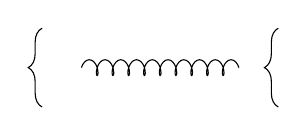
\begin{tikzpicture}
    % Draw the opening curly bracket {
    \draw[decorate,decoration={brace,amplitude=5pt,mirror}] (0, 0.5) -- (0, -0.5);

    % Draw the curly line with a label X on top
    \draw[decorate,decoration={coil,amplitude=1mm,segment length=2mm}] (0.5,0) -- (2.5,0) node[midway, above=2mm] {$\infinitesequences$};

    % Draw the closing curly bracket }
    \draw[decorate,decoration={brace,amplitude=5pt}] (3, -0.5) -- (3, 0.5);
\end{tikzpicture}
\caption{Fixpoint iterates of the maximal trace semantics.}
\labfig{iterates}
\end{marginfigure}

Intuitively, the iterates of the transformer $\tracetransformer$ starting from the set containing all infinite traces $\retrieveinfinitetraces{\state}$ are generated backwards by prepending transitions to them. In \reffig{iterates}, we illustrate the first few iterates of the transformer $\tracetransformer$.
Specifically, the finite traces are composed by extending finite traces from the final states $\finalstates$, one transition at a time, and the infinite traces are obtained by selecting infinite sequences with increasingly longer prefixes of transitions.
The $i$-th iterate of the transformer $\tracetransformer$ contains all finite traces of length at most $i$ that are terminating in the final states $\finalstates$, and all infinite sequences whose prefixes of length $i$ are generated by the transition relation $\transitionrelation$.
At the limit, we obtain the maximal trace semantics.

The maximal trace semantics is the most precise semantics and fully describes the behavior of programs. However, reasoning about a particular property of a program is often facilitated by the design of a semantics that abstracts away from irrelevant details about program computations.
In the following, to facilitate reading, we call the maximal trace semantics simply the \emph{trace semantics}.


\subsection{Collecting Semantics}
\labsec{collecting-semantics}

\marginnote{Program proerties are also reffered to as \emph{hyperproperties} \cite{Clarkson2010}. In this thesis, we prefer the term \emph{program properties} to emphasize that we consider properties of the semantics of programs.}
\phantomcite{Clarkson2010}
As seen in \refsec{properties}, a \emph{property} is specified by its extension, that is, the set of elements that manifest such property.
In this thesis, we consider \emph{program properties} with respect to their trace semantics.
By program property we mean properties of the semantics of programs.
In our settings, since the program semantics is the trace semantics in $\tracetype$, then a program property is a set of sets of traces in $\collectingtype$.
The strongest property of the trace semantics is the set containing the trace semantics and nothing else, this property is called the \emph{collecting semantics}.

\begin{definition}[Collecting Semantics]\labdef{collecting-semantics}
  Let $\tracesemanticsnoparam\in\tracetype$ be the trace semantics of a transition system $\transitionsystem$. The \emph{collecting semantics} $\collectingsemanticsnoparam\in\collectingtype$ is defined as:
  \begin{align*}
    \collectingsemanticsnoparam &\DefeQ \{\spacearound{\tracesemanticsnoparam}\}
  \end{align*}
\end{definition}

The collecting semantics $\collectingsemanticsnoparam$ is satisfied only and exactly by the trace semantics $\tracesemanticsnoparam$.
We write $\tracesemantics$ to denote the trace semantics of a particular program $\defprogram$, the same applies for the rest of semantics we study in this thesis. Hence, the collecting semantics of a program $\defprogram$ is denoted by $\collectingsemantics$.

\paragraph{Property Validation.}

A program $\defprogram$ with semantics $\tracesemantics$ satisfies a property $\defproperty \in \collectingtype$ if and only if the property $\defproperty$ is implied by the collecting semantics $\collectingsemantics\in\collectingtype$.


\begin{definition}[Validation of Program Properties]\labdef{validation}
  Let $\defprogram$ be a program and $\defproperty$ be a property of programs. We say that $\defprogram$ \emph{satisfies} $\defproperty$ whenever:
  \begin{align*}
    \defprogram \satisfies \defproperty \IfF \collectingsemantics \subseteq \defproperty
  \end{align*}
\end{definition}

Traditional properties are often trace properties, and thus can be expressed as sets of traces in $\tracetype$. In this case, it is often used a weaker form of property validation. A program $\defprogram$ satisfies a trace property $\defproperty\in\tracetype$ whenever the trace semantics $\tracesemantics$ implies the property $\defproperty$, not the collecting semantics. Note that, not all program properties can be expressed as trace properties. As an example, the unused property \sidecite{Urban2018} (\cf{} \refch{input-data-usage}) is not a trace property, because whether a program utilizes a variable or not depends on the whole set of traces generated by the program.

\paragraph{Hierarchy of Semantics}

To reason about a particular program property, it is not necessary to consider all the details of the trace semantics.
In fact, reasoning is facilitated by the design of an abstract semantics that forgets irrelevant details about program computations.
Therefore, there is no general purpose program semantics that is suitable for reasoning about all program properties.
Instead, there exist a wide range of program semantics dedicated to a specific class of program properties, each of them abstracting away from the computational details differently.

Abstract interpretation provides a systematic and uniform way to relate semantics described as fixpoints of monotonic functions over ordered structures.
These semantics are organized in a hierarchy, where the collecting semantics is the most precise semantics and all other semantics interrelate at different levels \sidecite{Cousot2002,Cousot2024b}.


\subsection{Galois Connection}
\labsec{galois-connection}

The corespondence between the semantics in the hierarchy is established by Galois connections formalizing the abstraction relation between the semantics.


\subsection{Reachable State Semantics}
\labsec{reachable-state-semantics}

\subsection{Fixpoint Transfer}
\labsec{fixpoint-transfer}

\subsection{Fixpoint Approximation}
\labsec{fixpoint-approximation}

\subsection{Widening}
\labsec{widening}

\subsection{Narrowing}
\labsec{narrowing}


\section{A Small Imperative Language}
\labsec{a-small-imperative-language}

\subsection{Syntax}
\labsec{syntax}

\subsection{Maximal Trace Semantics}
\labsec{maximal-trace-semantics}


\begin{definition}[State]\labdef{state}
  \begin{align*}
    \state \IN \variables \to \values
  \end{align*}
\end{definition}

\subsection{Numerical Abstract Domains}
\labsec{numerical-abstract-domains}

\subsubsection*{Sign}

\subsubsection*{Boxes}

\subsubsection*{Conjunctions of Linear Constraints}

\subsection{Reduced Product}
\labsec{reduced-product}

\subsection{Forward Reachability State Semantics}
\labsec{forward-reachability-state-semantics}

\subsection{Backward Reachability State Semantics}
\labsec{backward-reachability-state-semantics}

\begin{definition}[Validation]
  \labdef{validation}
  \begin{align}
    \labeq{validation}
    \defprogram \satisfies \defproperty \iff \collectingsemantics \subseteq \defproperty
  \end{align}
\end{definition}

\begin{definition}[Collecting Semantics]
  \labdef{collecting-semantics}
  \begin{align}
    \labeq{collecting-semantics}
    \collectingsemanticsnoparam \defeq \{ \dependencysemanticsnoparam \}
  \end{align}
\end{definition}

\begin{definition}[Dependency Semantics]
  \labdef{dependency-semantics}
  \begin{align*}
    \dependencysemanticsnoparam \DefeQ \setdef{\inputoutputtuple{\defseq}}{\defseq\in\tracesemanticsnoparam}
  \end{align*}
\end{definition}

\begin{definition}[Backward Semantics]\labdef{backward-semantics}
\begin{align*}
&\backwardsemanticsnoparam \semanticsof{\skipstmt}\defabstractvalue \DefeQ
\defabstractvalue
\\
&\backwardsemanticsnoparam \semanticsof{\assignstmt}\defabstractvalue \DefeQ
\abstractdomainsubstitute{\defvariable}{\defaexp}\defabstractvalue
\\
&\backwardsemanticsnoparam \semanticsof{\assertstmt}\defabstractvalue \DefeQ
\abstractdomainfilter\semanticsof{\defbexp}\defabstractvalue
\\
&\backwardsemanticsnoparam \semanticsof{\ifstmt[\defstmt][\defstmt']}\defabstractvalue \DefeQ
\\
&\quad \abstractdomainfilter\semanticsof{\defbexp}(\backwardsemanticsnoparam \semanticsof{\defstmt}\defabstractvalue) \spacearound{\abstractdomainjoin} \abstractdomainfilter\semanticsof{\neg\defbexp}(\backwardsemanticsnoparam \semanticsof{\defstmt'}\defabstractvalue)
\\
&\backwardsemanticsnoparam \semanticsof{\whilestmt}\defabstractvalue \DefeQ \lim_n \abstractdomainfixpoint_n \\
&\quad \abstractdomainfixpoint_0 \DefeQ \defabstractvalue \\
&\quad \abstractdomainfixpoint_{n+1} \DefeQ \abstractdomainfixpoint_n \spacearound{\abstractdomainwidening} \abstractdomainfixpoint(\abstractdomainfixpoint_n) \\
&\quad \abstractdomainfixpoint(\defotherabstractvalue) \DefeQ \abstractdomainfilter\semanticsof{\neg\defbexp}\defabstractvalue \spacearound{\abstractdomainjoin} \abstractdomainfilter\semanticsof{\defbexp}(\backwardsemanticsnoparam \semanticsof{\defstmt}\defotherabstractvalue)
\\
&\backwardsemanticsnoparam \semanticsof{\compstmt[\defstmt][\defstmt']}\defabstractvalue \DefeQ
\backwardsemanticsnoparam \semanticsof{\defstmt}( \backwardsemanticsnoparam \semanticsof{\defstmt'}\defabstractvalue)
\end{align*}
\end{definition}

\begin{marginlisting}
  \caption{Landing alarm system}
  \labprog{landing-alarm-system}
  \vspace{\lineheight}
\begin{lstlisting}[
  language=customPython,
  style=mystyle,]
landing_coeff =
  abs(angle) + speed
if landing_coeff < 2:
  risk = 0
else if landing_coeff > 5:
  risk = 3
else:
  risk =
    floor(landing_coeff) - 2
  \end{lstlisting}
\end{marginlisting}
